\documentclass[10pt, landscape]{article}
\usepackage[scaled=0.92]{helvet}
\usepackage{calc}
\usepackage{multicol}
\usepackage{ifthen}
\usepackage[a4paper,margin=3mm,landscape]{geometry}
\usepackage{amsmath,amsthm,amsfonts,amssymb}
\usepackage{color,graphicx,overpic}
\usepackage{hyperref}
\usepackage{newtxtext} 
\usepackage{enumitem}
\usepackage{amssymb}
\usepackage[table]{xcolor}
\usepackage{vwcol}
\usepackage{tikz}
\usetikzlibrary{arrows.meta}
\usetikzlibrary{calc}
\usepackage{mathtools}
\usepackage{nicematrix}
%For pictures / figures
\usepackage{color,graphicx,overpic}
\graphicspath{ {./images/} }
% for relations
\usepackage{cancel}
\usepackage{ mathrsfs }
\graphicspath{ {./images/} }
\setlist{nosep}
\usepackage{amssymb}  % For \checkmark


\pdfinfo{
  /Title (CG2271-Midterm-Cheatsheet.pdf)
  /Creator (TeX)
  /Producer (pdfTeX 1.40.0)
  /Author (Seamus)
  /Subject (Example)
  /Keywords (pdflatex, latex,pdftex,tex)}

% Turn off header and footer
\pagestyle{empty}

\newenvironment{tightcenter}{%
  \setlength\topsep{0pt}
  \setlength\parskip{0pt}
  \begin{center}
}{%
  \end{center}
}

% redefine section commands to use less space
\makeatletter
\renewcommand{\section}{\@startsection{section}{1}{0mm}%
                                {-1ex plus -.5ex minus -.2ex}%
                                {0.5ex plus .2ex}%x
                                {\normalfont\large\bfseries}}
\renewcommand{\subsection}{\@startsection{subsection}{2}{0mm}%
                                {-1explus -.5ex minus -.2ex}%
                                {0.5ex plus .2ex}%
                                {\normalfont\normalsize\bfseries}}
\renewcommand{\subsubsection}{\@startsection{subsubsection}{3}{0mm}%
                                {-1ex plus -.5ex minus -.2ex}%
                                {1ex plus .2ex}%
                                {\normalfont\small\bfseries}}%
\renewcommand{\familydefault}{\sfdefault}
\renewcommand\rmdefault{\sfdefault}
% makes nested numbering (e.g. 1.1.1, 1.1.2, etc)
\renewcommand{\labelenumii}{\theenumii}
\renewcommand{\theenumii}{\theenumi.\arabic{enumii}.}
\renewcommand\labelitemii{•}
%  for logical not operator
\renewcommand{\lnot}{\mathord{\sim}}
\renewcommand{\bf}[1]{\textbf{#1}}
\newcommand{\abs}[1]{\vert #1 \vert}
\newcommand{\Mod}[1]{\ \mathrm{mod}\ #1}

\makeatother
\definecolor{myblue}{cmyk}{1,.72,0,.38}
\everymath\expandafter{\the\everymath \color{myblue}}
% Define BibTeX command
\def\BibTeX{{\rm B\kern-.05em{\sc i\kern-.025em b}\kern-.08em
    T\kern-.1667em\lower.7ex\hbox{E}\kern-.125emX}}
\let\iff\leftrightarrow
\let\Iff\Leftrightarrow
\let\then\rightarrow
\let\Then\Rightarrow

% Don't print section numbers
\setcounter{secnumdepth}{0}

\setlength{\parindent}{0pt}
\setlength{\parskip}{0pt plus 0.5ex}
%% this changes all items (enumerate and itemize)
\setlength{\leftmargini}{0.5cm}
\setlength{\leftmarginii}{0.5cm}
\setlist[itemize,1]{leftmargin=2mm,labelindent=1mm,labelsep=1mm}
\setlist[itemize,2]{leftmargin=4mm,labelindent=1mm,labelsep=1mm}

%My Environments
\newtheorem{example}[section]{Example}
% -----------------------------------------------------------------------

\begin{document}
\raggedright
\footnotesize
\begin{multicols}{4}


% multicol parameters
% These lengths are set only within the two main columns
\setlength{\columnseprule}{0.25pt}
\setlength{\premulticols}{1pt}
\setlength{\postmulticols}{1pt}
\setlength{\multicolsep}{1pt}
\setlength{\columnsep}{2pt}

\begin{center}
    \fbox{%
        \parbox{0.8\linewidth}{\centering \textcolor{black}{
            {\Large\textbf{CG2271 Midterm}}
            \\ \normalsize{AY26/27 sem 1}}
            \\ {\footnotesize \textcolor{myblue}{github.com/mendax1234}} 
        }%
    }
\end{center}

\section{Intro to OS}
\begin{enumerate}
    \item OS is nothing special but a program which does
    \begin{itemize}
        \item virtualization of CPU via context switch and scheduling; virtualization of memory via giving each process a private address space
        \item solving the issues related to concurrency
        \item storing files persistently.
    \end{itemize}
    \item MIPS Instructions table: \\
    %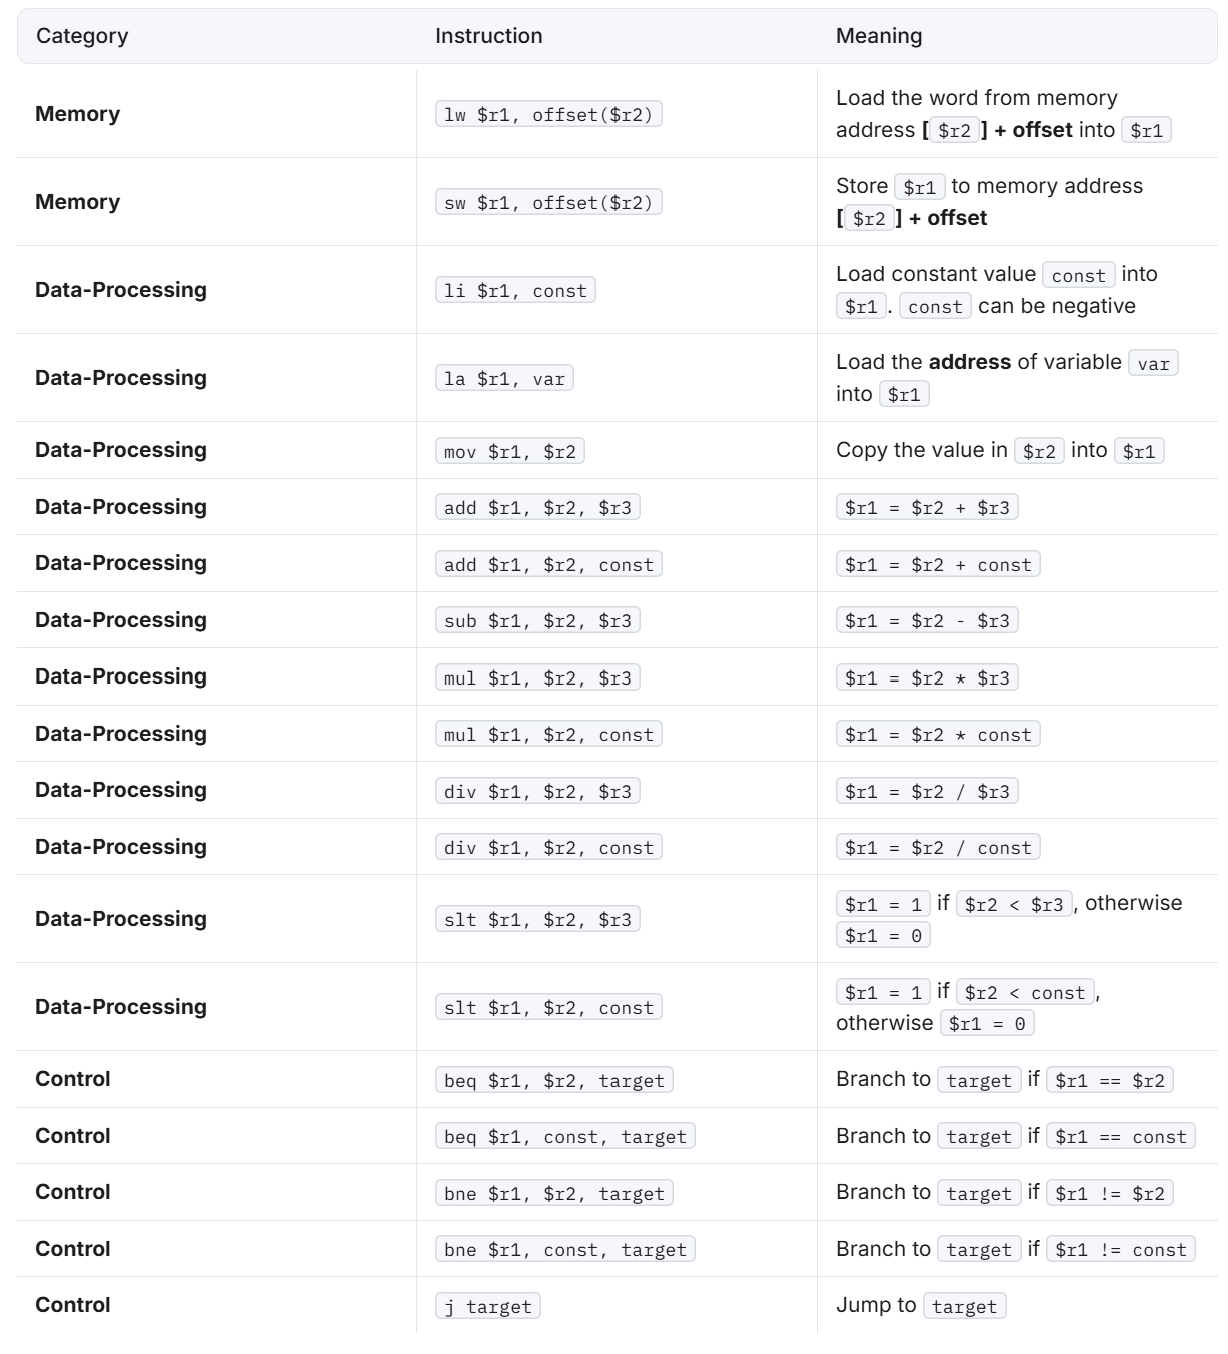
\includegraphics[width=1\linewidth]{images/midterm/2.png}
    {\centering
    \footnotesize
    \setlength{\tabcolsep}{2.5pt}
    \renewcommand{\arraystretch}{1.1}
    \begin{tabular}{l p{0.45\columnwidth}}
    \hline
    \textbf{Instruction} & \textbf{Meaning} \\
    \hline
    \texttt{lw \$r1, offset(\$r2)} & Load word from \textbf{[\texttt{\$r2}] + offset} into \texttt{\$r1} \\
    \texttt{sw \$r1, offset(\$r2)} & Store \texttt{\$r1} to \textbf{[\texttt{\$r2}] + offset} \\
    \hline
    \texttt{li \$r1, const} & Load constant \texttt{const} into \texttt{\$r1} (can be negative) \\
    \texttt{la \$r1, var} & Load address of \texttt{var} into \texttt{\$r1} \\
    \texttt{mov \$r1, \$r2} & Copy \texttt{\$r2} into \texttt{\$r1} \\
    \texttt{add \$r1, \$r2, \$r3} & \texttt{\$r1 = \$r2 + \$r3} \\
    \texttt{add \$r1, \$r2, const} & \texttt{\$r1 = \$r2 + const} \\
    \texttt{sub \$r1, \$r2, \$r3} & \texttt{\$r1 = \$r2 - \$r3} \\
    \texttt{mul \$r1, \$r2, \$r3} & \texttt{\$r1 = \$r2 * \$r3} \\
    \texttt{mul \$r1, \$r2, const} & \texttt{\$r1 = \$r2 * const} \\
    \texttt{div \$r1, \$r2, \$r3} & \texttt{\$r1 = \$r2 / \$r3} \\
    \texttt{div \$r1, \$r2, const} & \texttt{\$r1 = \$r2 / const} \\
    \texttt{slt \$r1, \$r2, \$r3} & \texttt{\$r1 = 1} if \texttt{\$r2 < \$r3}, else \texttt{0} \\
    \texttt{slt \$r1, \$r2, const} & \texttt{\$r1 = 1} if \texttt{\$r2 < const}, else \texttt{0} \\
    \hline
    \texttt{beq \$r1, \$r2, tgt} & Branch to \texttt{tgt} if \texttt{\$r1 == \$r2} \\
    \texttt{beq \$r1, const, tgt} & Branch to \texttt{tgt} if \texttt{\$r1 == const} \\
    \texttt{bne \$r1, \$r2, tgt} & Branch to \texttt{tgt} if \texttt{\$r1 != \$r2} \\
    \texttt{bne \$r1, const, tgt} & Branch to \texttt{tgt} if \texttt{\$r1 != const} \\
    \texttt{j tgt} & Jump to \texttt{tgt} \\
    \hline
    \end{tabular}\par}
    \begin{itemize}
        \item For control instructions, \texttt{target} usually refers to a label, which identifies the location to jump or branch to.
        \item \texttt{lw} is used to read a variable's value from memory into a register, e.g., \texttt{lw \$1, x} is used to load the variable \texttt{x}'s value into register 1. After modifying the value, \texttt{sw} is used to write the updated value back to memory.
        \item The usual flow for writing a decision in assembly is:
        \begin{enumerate}
            \item Set up the condition check, usually using \texttt{slt}.
            \item Branch to the \texttt{else} part if the condition is false.
            \item Execute the \texttt{if} part if the condition is true and remember to jump to skip the else part.
            \item Continue after the else part using another label.
        \end{enumerate}
    \end{itemize}
    \item Variables declared \textbf{outside} \texttt{main()} are \textbf{global variables}, so they are stored in the \textbf{data memory region}.
    \item (\textbf{Monolithic Structure}): Since almost everything is in kernel mode, this structure has very \textbf{good performance}, but it is dangerous. \\
    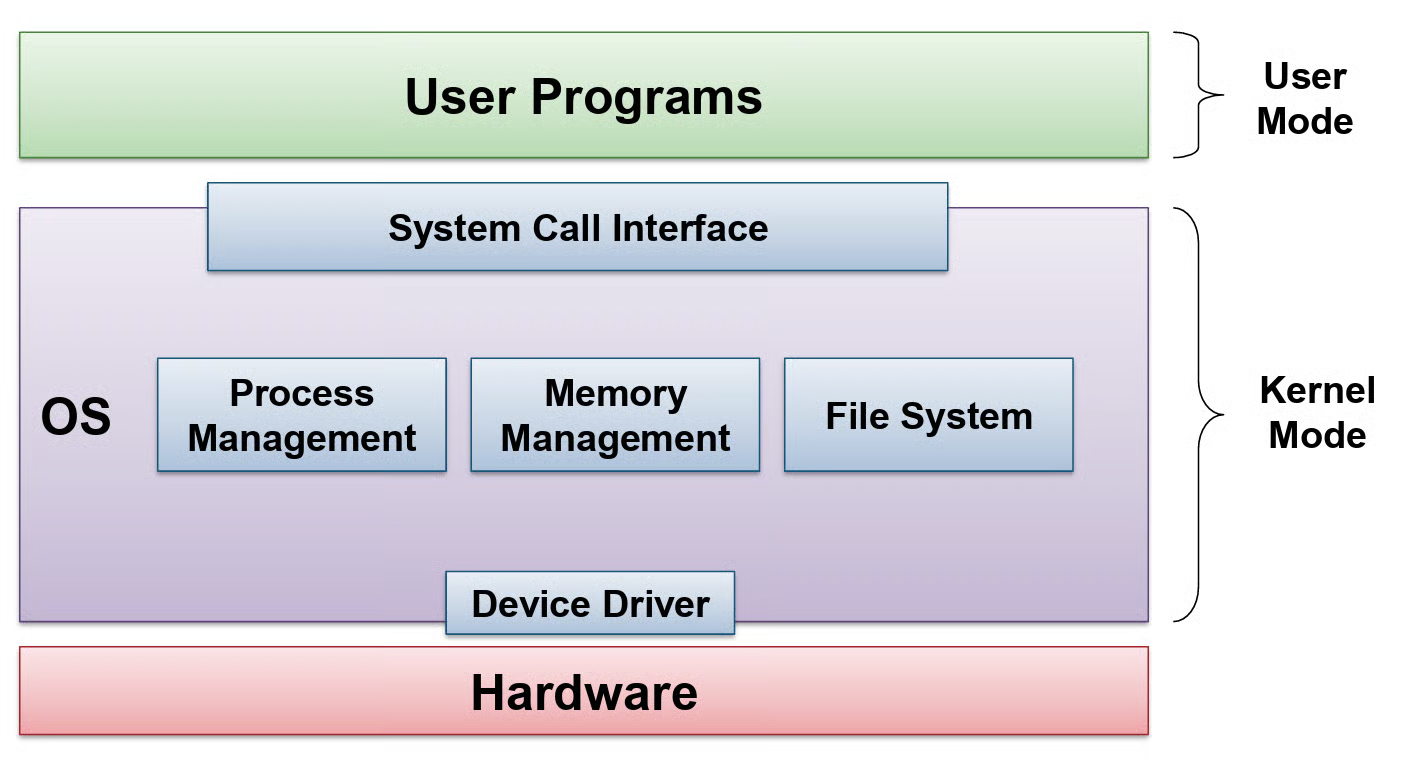
\includegraphics[width=1\linewidth]{images/midterm/4.png}
    \item (\textbf{Microkernel Structure}): All the higher level services are separate out, making the programs running in kernel mode very \textbf{small and clean}. However, the disadvantage is \textbf{low performance} as we need frequent context switches. \\
    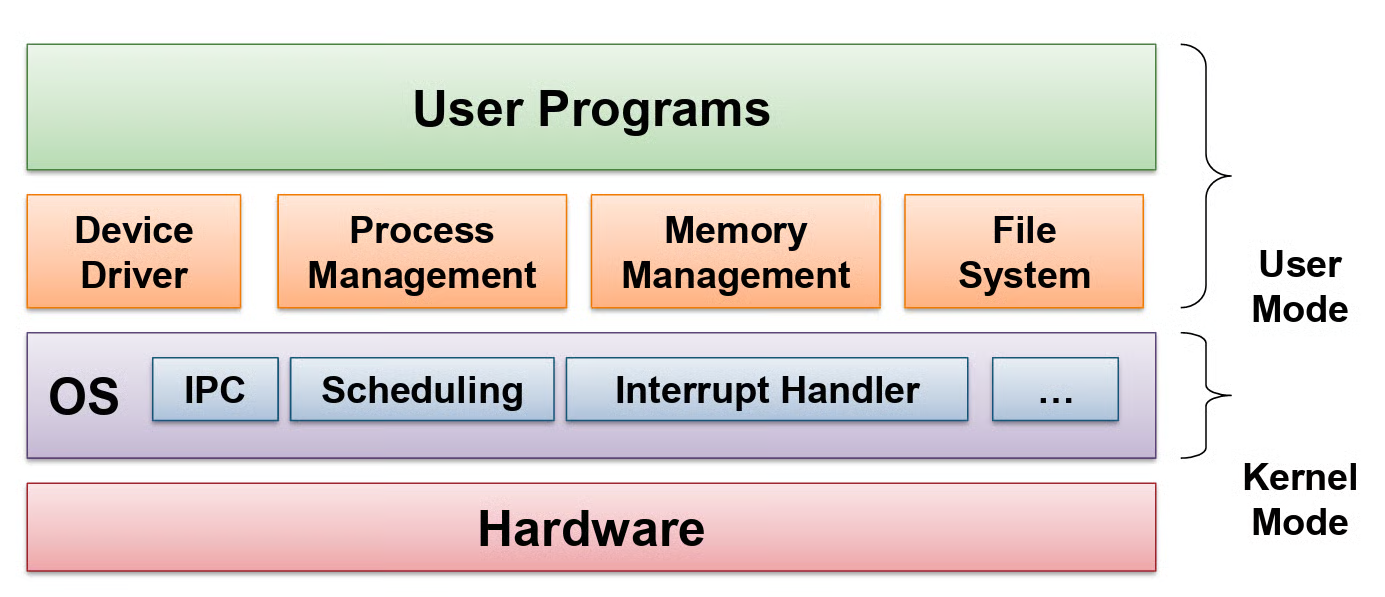
\includegraphics[width=1\linewidth]{images/midterm/5.png}
    \begin{itemize}
        \item It is \textbf{wrong} to say that in a monolithic OS, the entire kernel is compiled as a single large program.
        \item Microkernel OSes provide IPC mechanism to allow communication between programs in user mode and kernel mode.
        \item Process scheduler runs in \textbf{kernel mode} in both monolithic and microkernel OSes!
    \end{itemize}
    \item \textbf{ISR:} handles hardware interrupts and notifies the OS of events (e.g.\ I/O completion), allowing waiting processes to move \textbf{Blocked $\rightarrow$ Ready}.
    \item \textbf{OS:} virtualizes/abstracts hardware for processes.
    \item \textbf{Hypervisor:} virtualizes hardware for multiple \textbf{guest operating systems / VMs}.
    \item \textbf{Types of VMs}: Type 1 hyperviser sits on top of the \textbf{hardware} while type 2 hypervisor sits on top of a \textbf{host OS}.
    \item \textbf{Attention:} Uninitialized local variables read residual (dirty) values from whichever prior frame data shared that exact stack slot.
\end{enumerate}

\section{Process Abstraction}
\begin{enumerate}
    \item The machine state of a process contains the following 3 contexts which are stored in the \textbf{process control block (PCB)} (except for memory context)
    \begin{itemize}
        \item Memory Context: Code, Data, Stack, Heap. PCB does \textbf{not} store actual memory contents (Code, Data, Heap, Stack). PCB stores \textbf{memory-management information/pointers} needed to locate and manage the process's address space.
        \item Hardware Context: Registers, PC, $\dots$
        \item OS Context: Process Properties, Resources used
    \end{itemize}
    \item Each process has its own address space, namely memory context.
    \item (\textbf{User Stack}): The user stack is a region of memory used to store information associated with function calls. Each function invocation is represented by a stack frame.
    \item (\textbf{User Stack Pointer}): This pointer always points to the top of the user stack for a given process.
    \item In C, it is impossible for a callee to access the variables in the caller that are not passed to callee!
    \item (\textbf{Frame pointer}): A frame pointer always points to the bottom (start) of the current stack frame, making it easier to access the local variables and arguments passed from the caller because their offsets from the frame pointer remain fixed.
    \item (\textbf{Process Table}): The Process Table can be thought of as a data structure maintained by the kernel that contains an entry for every process. \textbf{Each entry is a PCB}, which is why a PCB is also referred to as a \textbf{process table entry (PTE)}.
    \item The process table and PCB both reside in \textbf{kernel space}, while the process's actual memory space resides in \textbf{user space}.
    \item Typically, to calculate the stack frame's size when calling a function, we should consider:
    \begin{itemize}
        \item \textbf{Return address / PC}: where execution resumes.
        \item \textbf{Saved old FP}: restores caller's frame pointer.
        \item \textbf{Saved old SP}: if required by the calling convention.
        \item \textbf{Parameters}: if passed on the stack.
        \item \textbf{Local variables}: variables declared inside the function.
        \item \textbf{Return-value space}: if stored on the stack.
        \item \textbf{Saved registers}: temporary registers that must be preserved.
    \end{itemize}
    \item A calling convention that allocates a fixed 4 bytes per parameter/local does \textbf{not} support arbitrary data types. To support any type, allocate stack space according to each variable's \textbf{size and alignment}; large objects may be passed by pointer.
    \item A calling convention example:\par
    {\centering
    \begin{tabular}{ll}
    \hline
    \textbf{Value stored} & \textbf{Location} \\
    \hline
    Saved old FP & $FP$ \\
    Saved old SP & $FP+4$ \\
    Return address & $FP+8$ \\
    Parameter 1 & $FP+12$ \\
    Parameter 2 & $FP+16$ \\
    $\vdots$ & $\vdots$ \\
    Parameter $n$ & $FP+4(n+3)$ \\
    Return value & $FP+4(n+4)$ \\
    Start of local-variable area & $FP+4(n+5)$ \\
    Local variables & $FP+4(n+5)$ to $SP$ \\
    \hline
    \end{tabular}\par}
    \begin{itemize}
        \item \textbf{Caller} allocates the basic frame up to $FP+4(n+5)$.
        \item \textbf{Callee} extends $SP$ by $4m$ bytes to reserve space for its local variables. ($m$ denotes the number of local variables)
    \end{itemize}
    \item (\texttt{fork()}): When a process calls \texttt{fork()}, the OS creates a new process by copying the parent process's PCB, including its hardware, OS, and memory contexts. The OS context is then updated with a new PID, while the child continues executing the same code from the point immediately after \texttt{fork()}.
    \begin{itemize}
        \item A successful call to \texttt{fork()} always \textbf{doubles} the number of executing processes. (The problem of ``fork-bomb'').
        \item The return value of \texttt{fork()} differs between the parent and child process:
        \begin{itemize}
            \item Child process: \texttt{fork()} returns 0.
            \item Parent process: \texttt{fork()} returns the \textbf{PID} ($>$0) of the newly created child.
            \item \textbf{\texttt{-1}}: Indicates failure; no child is created, and \texttt{errno} is set.
        \end{itemize}
        \item After each \texttt{fork()}, the parent and child have separate copies of their \textbf{local and global variables}. Changes to these variables in one process do not affect the other, allowing each process to maintain independent state.
    \end{itemize}
    \item (\textbf{Process State Transition}): \\
    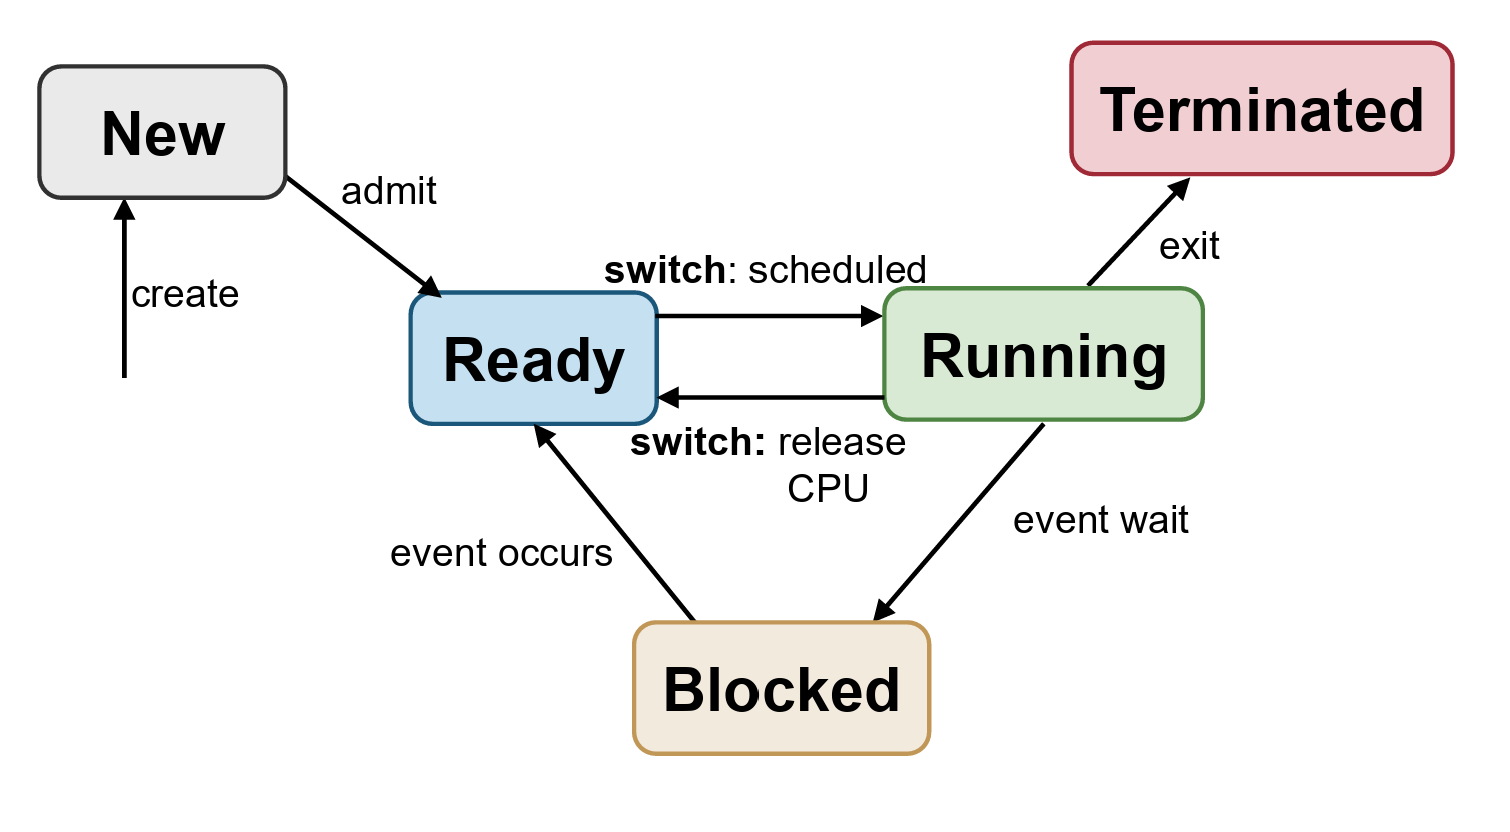
\includegraphics[width=1\linewidth]{images/midterm/7.png}
\end{enumerate}

\section{Process Scheduling}
\begin{enumerate}
    \item (\textbf{Turnaround time}): $T_{\text{turnaround}}=T_{\text{completion}}-T_{\text{arrival}}$
    \item (\textbf{Response time}): $T_{\text{response}}=T_{\text{firstrun}}-T_{\text{arrival}}$
    \item (\textbf{RTOS Scheduling}): RTOS scheduling can be classified by how task priorities are assigned. We normally assume \textbf{pre-emption is enabled} and \textbf{time-slicing is disabled}.
    \begin{itemize}
        \item \textbf{Fixed-Priority Scheduling}: Each task is assigned a fixed priority that does not change.
        \item \textbf{Rate Monotonic Scheduling (RMS)}: A fixed-priority scheme where priority is determined by the task's \textbf{period}; a shorter period gives a higher priority.
        \item \textbf{Earlier Deadline First (EDF)} scheduling: This is not a fixed priority scheduling scheme, a task's priority is increased as its deadline approaches.
        \item If CPU utilization is under 100\%, EDF always guarantees schedulability.
        \item \textbf{Deadlines}: A task's deadline is the \textbf{latest time by which it must finish}. In periodic real-time tasks, the deadline is often equal to the task's \textbf{period}, meaning one instance should finish before the next instance is released.
    \end{itemize}
    \item (\textbf{Liu and Layland Bound}: This is to check if a set of tasks is schedulable under RMS. A set of $n$ periodic tasks is guaranteed to be schedulable under RMS if $U \leq n\left(2^{1/n}-1\right)$, where $U=\sum_i\frac{C_i}{P_i}$. Tasks that fail to meet L\&L bound may still be schedulable under RMS.
    \item (\textbf{Critical Instance Analysis}: It tests the schedulability systematically by computing the worst-case response time of each task.
    \begin{itemize}
        \item Sort the tasks by period: If the tasks are not already sorted, arrange them in increasing order of period. Thus, $T_1$ has the shortest period, $T_2$ the second shortest, and so on.
        \item For each task $T_i$, recursively compute $S_{i,0}, S_{i,1}, \ldots$
        \item $S_{i,0} = \sum_{j=1}^{i} C_j$: This represents the initial workload when all higher-priority tasks and $T_i$ are released simultaneously.
        \item $S_{i,x+1} = C_i + \sum_{j=1}^{i-1} \left\lceil \frac{S_{i,x}}{P_j} \right\rceil C_j$: The summation accounts for the preemptions caused by higher-priority tasks. Continue until $S_{i,x+1} = S_{i,x}$ and call this final value $S_{i,F}$. ($x+1$ can be greater than $i$)
        \item Check the deadline: $S_{i,F} \le D_i$. If this condition holds for every task $T_i$, then the entire task set is schedulable under RMS and no task will miss its deadline.
        \item (\textbf{Tips}): Usually we start with the \textbf{lowest-priority task} first.
    \end{itemize}
    \item \textbf{Example: Critical Instant Analysis (RMS)}
    \begin{tabular}{c|cc}
    \hline
    \textbf{Task} & \textbf{Period }$P_i$ & \textbf{Execution Time }$C_i$ \\
    \hline
    $T_1$ & 6 & 2 \\
    $T_2$ & 8 & 2 \\
    $T_3$ & 4 & 1 \\
    \hline
    \end{tabular}
    
    \begin{itemize}
        \item Under RMS, sort by increasing period:
              $\{T_3,T_1,T_2\}$, so $T_2$ is the \textbf{lowest-priority task}.
        \item \textbf{Check $T_2$:}
        \[
        S_{2,0}=C_3+C_1+C_2=1+2+2=5
        \]
        \[
        S_{2,1}=C_2+\left\lceil\frac{5}{4}\right\rceil C_3
        +\left\lceil\frac{5}{6}\right\rceil C_1
        =2+2+2=6
        \]
        \[
        S_{2,2}=2+\left\lceil\frac{6}{4}\right\rceil(1)
        +\left\lceil\frac{6}{6}\right\rceil(2)=6
        \]
        Since $S_{2,2}=S_{2,1}=6\leq P_2=8$, $T_2$ is schedulable.
        \item Since the \textbf{lowest-priority task is schedulable}, the higher-priority tasks $T_1$ and $T_3$ are also schedulable.
    \end{itemize}
    \item (\textbf{Pre-emptive} Priority Scheduling): In this scheme, don't use the idea of ready queue, if need, the ready queue is prioritized!
    \item In this course, we made the following conventions when scheduling tasks (Please refer to the actual Test)
    \begin{itemize}
        \item The task that arrives earlier is scheduled first. Also, if multiple ready processes have the same remaining time, break the tie by \textbf{ready-queue order}: the process that joined/rejoined the ready queue \textbf{earlier} runs first.
        \item If two tasks arrive at the same time, choose the task according to alphabetical order if they have the same priority. Otherwise, higher priority first.
        \item A task arriving at time $x$ becomes ready exactly at time $x$ (on the horizontal axis), as illustrated below.
        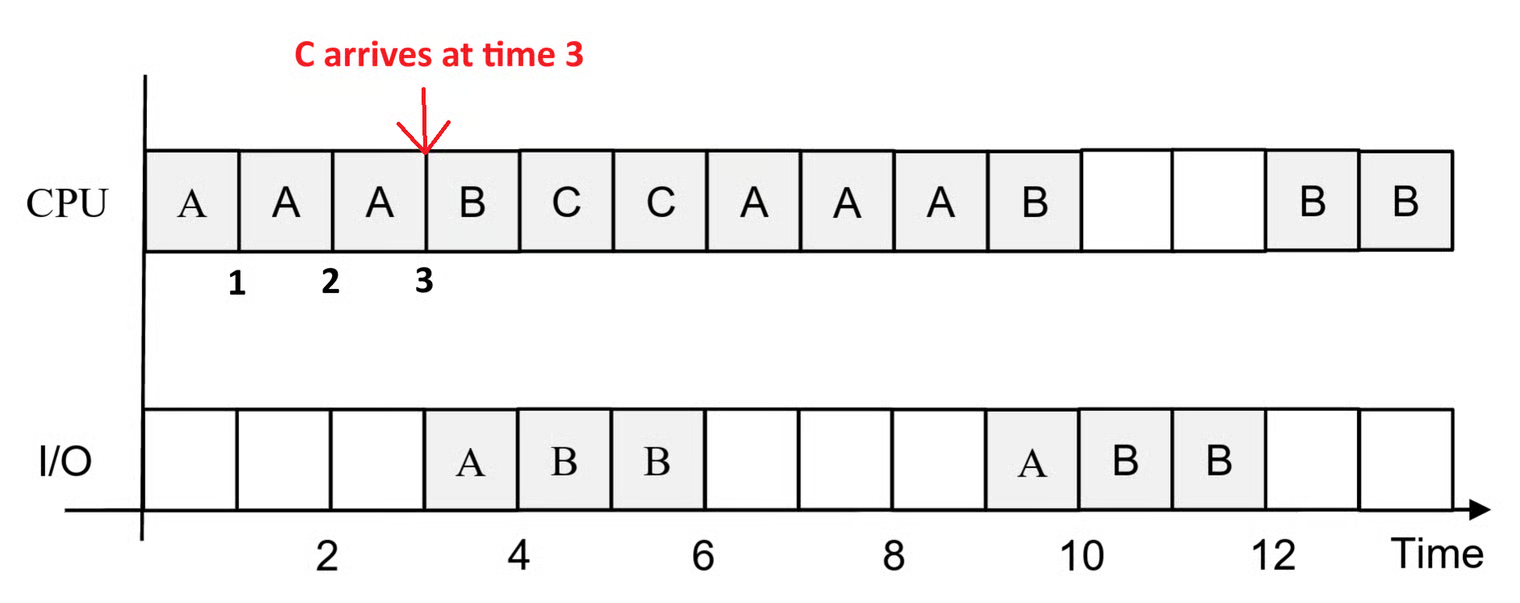
\includegraphics[width=1\linewidth]{images/midterm/3.png}
        \item When calculating turnaround time, use the R.H.S coordinates. When calculating the response time, use the L.H.S coordinates. for the scheduling above, assume B arrives at time 1.
        \begin{tabular}{c|cc}
        \hline
        \textbf{Process} & \textbf{Turnaround Time} & \textbf{Response Time} \\
        \hline
        A & 9  & 0 \\
        B & 13 & 2 \\
        C & 3  & 1 \\
        \hline
        \end{tabular}
    \end{itemize}
    
    \item (\textbf{Waiting Time}): $\text{Waiting Time}=\text{Turnaround Time}-\text{Service Time}$, where service time is the total time during which the task is actually running on the CPU or I/O.
    \item (\textbf{Round Robin} Scheduling): 
    \begin{itemize}
        \item If a process finishes before its time quantum expires, immediately schedule another ready process; the CPU does \textbf{not} wait for the remaining quantum. CPU is idle only if the ready queue is empty.
        \item \textbf{Round Robin is preemptive by time quantum:} a new arrival does \textbf{not} preempt the running process merely because it has higher priority.
        \item \textbf{Round Robin (RR)} maintains a \textbf{FIFO ready queue}. Each ready process runs for at most a fixed \textbf{time quantum}. If the quantum expires and the process is not finished, it is \textbf{preempted} and moved to the \textbf{back of the ready queue}.
    \end{itemize}
    \item We must take the \textbf{I/O} completion time also into account when calculating the turnaround time and waiting time!
    \item (\textbf{Shortest Job First (SJF) Scheduling}): The scheduler will run the \textbf{shortest} job first, then the \textbf{next shortest}, and so on.
    \item (\textbf{Incorporating I/O}): When incorporating the I/O into consideration for scheduling, it is recommended to draw the following diagram. Even without I/O, it is also recommended to draw the following diagram! \\
    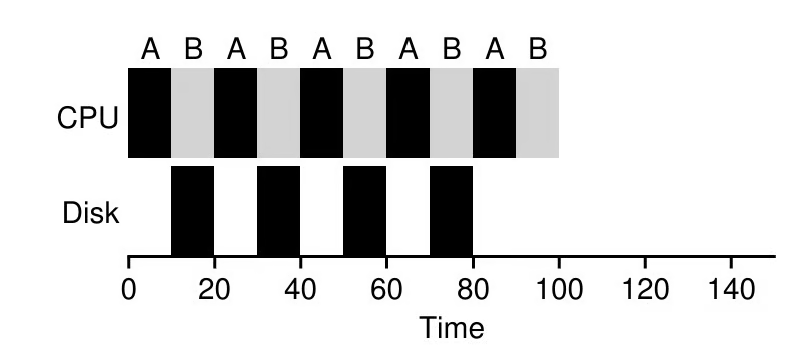
\includegraphics[width=1\linewidth]{images/midterm/6.png}
    \item When analyzing which scheduling algorithm is better, it's always a ``it depends'' question. So, one tip is to clearly compare the trade-off between turnaround time and response time.
\end{enumerate}

\section{Threads}
\begin{enumerate}
    \item Each thread has its own \textbf{hardware context}, which include registers and user stack (these user stacks will stay in the same stack memory region of the process, thus making the stack memory region fragmented).
    \begin{itemize}
        \item Each thread also has its own \textbf{thread-related OS context}: thread ID, state, priority, scheduling information, etc.
        \item Threads in the same process \textbf{share process-level OS resources} such as the address space and open files.
    \end{itemize}
    \item In C, each function call creates a stack frame on the thread's stack, and a function cannot directly access local variables stored in another stack frame unless they are explicitly passed to it or otherwise made accessible.
    \item (\textbf{User Thread}): A user thread is implemented by a thread library in user space, so the kernel is not aware of individual threads and it only sees a process is running. The library and its runtime system manage thread creation, switching, and scheduling.
    \begin{itemize}
        \item Advantages: thread operations are fast because they are just library calls, the scheduling policy can be customized, and user threads can run on almost any OS.
        \item Disadvantages: because the kernel schedules at the process level, one blocked thread can block the entire process, and the process cannot exploit multiple CPUs by running its threads in parallel.
    \end{itemize}
    \item (\textbf{Kernel Thread}): A kernel thread is implemented and managed by the OS. Thread operations are handled through system calls, and the kernel can schedule individual threads. In other words, the kernel now has the knowledge of which thread within a process is runnable. \textbf{However}, the trade-off is that thread operations are more expensive because they require kernel involvement, and the implementation is generally less flexible.
    \item Threads are ``lightweight processes'' because they have \textbf{less creation/context-switch overhead} than full processes.
    \item Pthread API
        \begin{itemize}
        \item \texttt{pthread\_create(\&tid, NULL, func, arg)}: starts a thread running \texttt{func(arg)}.
        \item The \texttt{pthread\_create} returns 0 to indicate success and !0 to indicate errors.
        \item Thread function format: \texttt{void *func(void *arg)}.
        \item \texttt{pthread\_exit(ret)}: terminates the thread and returns \texttt{ret}.
        \item \texttt{pthread\_join(tid, \&ret)}: waits for the thread; stores the thread's return value in \texttt{ret}. This is called thread synchronization. Without it, the child thread might terminate when its parent process finishes executing. To let the parent process wait for its child, we should use this API.
        \item \texttt{pthread\_join()} itself returns \textbf{0 on success}, not the thread's return value.
    \end{itemize}
\end{enumerate}

\section{Inter-Process Communication}
\begin{enumerate}
    \item (\textbf{Synchronization}): The send or receive operation blocks the process until the required communication can take place. For example
    \begin{itemize}
        \item The read process waits until the pipe is not empty then it will start reading.
        \item The write process waits until the pipe is not full when it will start writing.
    \end{itemize}
    \item \textbf{Shared-memory race:} processes created by \texttt{fork()} can access the same shared-memory object. If multiple processes write the same location without synchronization, the final value is \textbf{non-deterministic}.
    \item Shared Memory API:
    \begin{itemize}
    \item \texttt{shmid = shmget(key, size, flags)}: create/get a shared-memory segment $\rightarrow$ \texttt{shmid}.
    \begin{itemize}
        \item \texttt{key}: identifies the shared-memory segment.
        \item \texttt{size}: allocate space for $N$ elements using \texttt{N * sizeof(type)}.
        \item \texttt{flags}: e.g.\ \texttt{IPC\_CREAT | 0600}; \texttt{0} indicates octal notation, and \texttt{6 = rw-} gives the owner read/write permission while the two \texttt{0}s give group and others no permission. If we use hex, it will be \texttt{0x180}.
    \end{itemize}
        \item \texttt{shm = shmat(shmid,...)}: attaches a shared-memory segment to a pointer in user space so that we can use the pointer to access the shared memory. The shared-memory segment itself is managed by the kernel and thus living in the kernel space.
        \begin{itemize}
            \item After attach, can use \texttt{shm[0,$\dots$,N-1]} to access the value in the shared memory region if we want to create an array in the shared memory region.
        \end{itemize}
        \item Access shared memory normally through the returned pointer.
        \item \texttt{shmdt(ptr)}: detach shared memory.
        \item \texttt{shmctl(shmid, IPC\_RMID, NULL)}: delete shared-memory segment.
    \end{itemize}
    \item (\textbf{UNIX Pipe}):
    \begin{itemize}
        \item Pipe ends: \texttt{fd[0]} = read, \texttt{fd[1]} = write.
        \item Writer closes \texttt{fd[0]}; reader closes \texttt{fd[1]}.
        \item Empty pipe + write end still open $\Rightarrow$ \textbf{read blocks}.
        \item Empty pipe + all write ends closed $\Rightarrow$ \textbf{EOF}.
        \item Full pipe + blocking \texttt{write()} $\Rightarrow$ writer blocks; data is not simply lost.
        \item \texttt{dup2(fd[0], STDIN\_FILENO)} redirects \texttt{stdin} from the keyboard to the \textbf{pipe read end}.
        \item \texttt{dup2(fd[1], STDOUT\_FILENO)} redirects \texttt{stdout} from the screen to the \textbf{pipe write end}.
    \end{itemize}
\end{enumerate}

\section{Synchronization}
\begin{enumerate}
    \item \textbf{Semaphore Behaviour}:
    \begin{itemize}
        \item \texttt{wait(S)}: If $S \leq 0$, block; otherwise, $S \gets S-1$.
        \item \texttt{signal(S)}: $S \gets S+1$; wake up a waiting process, if any.
    \end{itemize}
    \item Deadlock can occur when processes acquire multiple semaphores in different orders, causing each process to wait for a resource held by the other. \\ 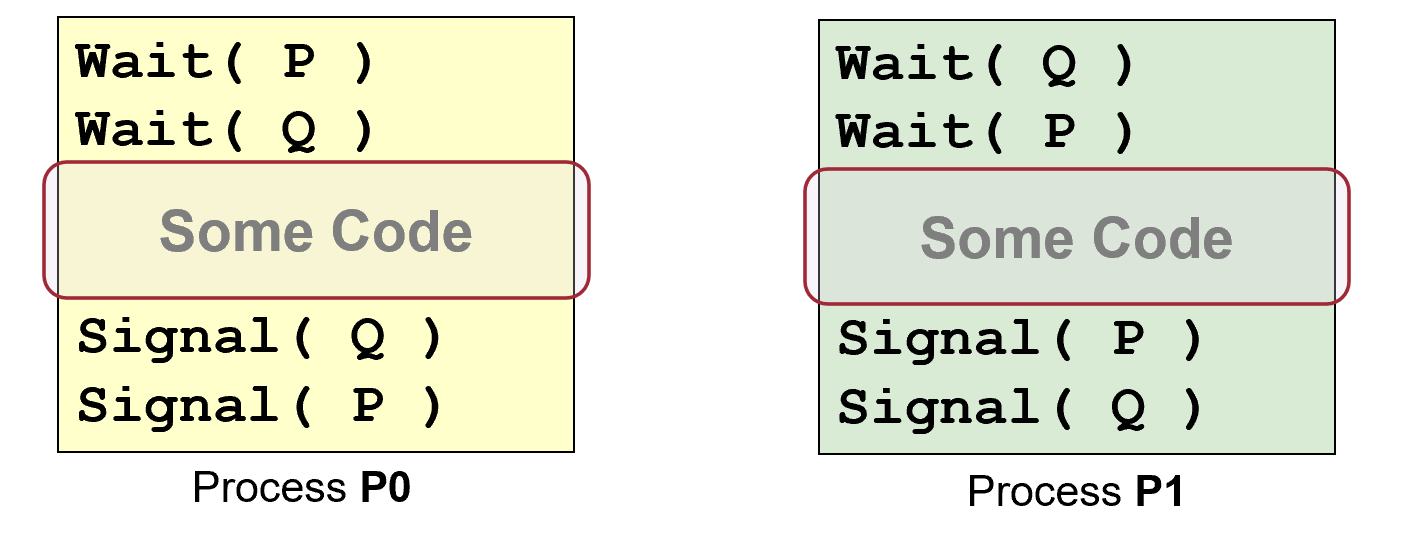
\includegraphics[width=1\linewidth]{images/midterm/1.png}
    \item The beauty of using semaphores is that it allows the thread blocked to sleep instead of busy waiting and consume the CPU resources uselessly.
    \item Binary semaphores are commonly used for mutual exclusion, while counting semaphores are used to track the number of available resources/conditions and block threads when none are available. For example, in the producer-consumer problem, we solve it using three semaphores:
    \begin{itemize}
        \item mutex = 1: ensures mutual exclusion when accessing the buffer.
        \item notFull = K: number of empty slots available.
        \item notEmpty = 0: number of items available to consume.
    \end{itemize}
    \item Operations that modify the state or value of a semaphore or mutex are performed atomically. The critical section doesn't need to be executed atomically!
    \item (\textbf{Mutex vs. Binary Semaphores})In NUS CG2271, or in FreeRTOS, the difference between mutex and a binary semaphore is that a mutex is nothing but a binary semaphore which is initialized to 1, while a binary semaphore in FreeRTOS is always intialized to 0.
    \item (\textbf{Conditional Variables vs. Counting Semaphores}): Conditional variables can wake up all the waiting process in the waiting queue through a mechanism called \texttt{broadcast}. While counting semaphores can at most wake up 1 process.
    \item (\textbf{Non-negative Semaphore}): In NUS CG2271, we use the convention that a semaphore's value is always non-negative. Therefore, the semaphore value does not indicate how many threads/processes are currently blocked because of this semaphore.
\end{enumerate}

\end{multicols}

% Dividing Line
% \hrulefill \\
% \begin{multicols}{4}
% \begin{enumerate}
% \end{enumerate}
% \end{multicols}

\end{document}